% Options for packages loaded elsewhere
\PassOptionsToPackage{unicode}{hyperref}
\PassOptionsToPackage{hyphens}{url}
\PassOptionsToPackage{dvipsnames,svgnames,x11names}{xcolor}
%
\documentclass[
  number,
  preprint,
  3p,
  twocolumn]{elsarticle}

\usepackage{amsmath,amssymb}
\usepackage{iftex}
\ifPDFTeX
  \usepackage[T1]{fontenc}
  \usepackage[utf8]{inputenc}
  \usepackage{textcomp} % provide euro and other symbols
\else % if luatex or xetex
  \usepackage{unicode-math}
  \defaultfontfeatures{Scale=MatchLowercase}
  \defaultfontfeatures[\rmfamily]{Ligatures=TeX,Scale=1}
\fi
\usepackage{lmodern}
\ifPDFTeX\else  
    % xetex/luatex font selection
\fi
% Use upquote if available, for straight quotes in verbatim environments
\IfFileExists{upquote.sty}{\usepackage{upquote}}{}
\IfFileExists{microtype.sty}{% use microtype if available
  \usepackage[]{microtype}
  \UseMicrotypeSet[protrusion]{basicmath} % disable protrusion for tt fonts
}{}
\makeatletter
\@ifundefined{KOMAClassName}{% if non-KOMA class
  \IfFileExists{parskip.sty}{%
    \usepackage{parskip}
  }{% else
    \setlength{\parindent}{0pt}
    \setlength{\parskip}{6pt plus 2pt minus 1pt}}
}{% if KOMA class
  \KOMAoptions{parskip=half}}
\makeatother
\usepackage{xcolor}
\setlength{\emergencystretch}{3em} % prevent overfull lines
\setcounter{secnumdepth}{5}
% Make \paragraph and \subparagraph free-standing
\ifx\paragraph\undefined\else
  \let\oldparagraph\paragraph
  \renewcommand{\paragraph}[1]{\oldparagraph{#1}\mbox{}}
\fi
\ifx\subparagraph\undefined\else
  \let\oldsubparagraph\subparagraph
  \renewcommand{\subparagraph}[1]{\oldsubparagraph{#1}\mbox{}}
\fi


\providecommand{\tightlist}{%
  \setlength{\itemsep}{0pt}\setlength{\parskip}{0pt}}\usepackage{longtable,booktabs,array}
\usepackage{calc} % for calculating minipage widths
% Correct order of tables after \paragraph or \subparagraph
\usepackage{etoolbox}
\makeatletter
\patchcmd\longtable{\par}{\if@noskipsec\mbox{}\fi\par}{}{}
\makeatother
% Allow footnotes in longtable head/foot
\IfFileExists{footnotehyper.sty}{\usepackage{footnotehyper}}{\usepackage{footnote}}
\makesavenoteenv{longtable}
\usepackage{graphicx}
\makeatletter
\def\maxwidth{\ifdim\Gin@nat@width>\linewidth\linewidth\else\Gin@nat@width\fi}
\def\maxheight{\ifdim\Gin@nat@height>\textheight\textheight\else\Gin@nat@height\fi}
\makeatother
% Scale images if necessary, so that they will not overflow the page
% margins by default, and it is still possible to overwrite the defaults
% using explicit options in \includegraphics[width, height, ...]{}
\setkeys{Gin}{width=\maxwidth,height=\maxheight,keepaspectratio}
% Set default figure placement to htbp
\makeatletter
\def\fps@figure{htbp}
\makeatother

\makeatletter
\@ifpackageloaded{caption}{}{\usepackage{caption}}
\AtBeginDocument{%
\ifdefined\contentsname
  \renewcommand*\contentsname{Table of contents}
\else
  \newcommand\contentsname{Table of contents}
\fi
\ifdefined\listfigurename
  \renewcommand*\listfigurename{List of Figures}
\else
  \newcommand\listfigurename{List of Figures}
\fi
\ifdefined\listtablename
  \renewcommand*\listtablename{List of Tables}
\else
  \newcommand\listtablename{List of Tables}
\fi
\ifdefined\figurename
  \renewcommand*\figurename{Figure}
\else
  \newcommand\figurename{Figure}
\fi
\ifdefined\tablename
  \renewcommand*\tablename{Table}
\else
  \newcommand\tablename{Table}
\fi
}
\@ifpackageloaded{float}{}{\usepackage{float}}
\floatstyle{ruled}
\@ifundefined{c@chapter}{\newfloat{codelisting}{h}{lop}}{\newfloat{codelisting}{h}{lop}[chapter]}
\floatname{codelisting}{Listing}
\newcommand*\listoflistings{\listof{codelisting}{List of Listings}}
\makeatother
\makeatletter
\makeatother
\makeatletter
\@ifpackageloaded{caption}{}{\usepackage{caption}}
\@ifpackageloaded{subcaption}{}{\usepackage{subcaption}}
\makeatother
\usepackage{float}
\makeatletter
\let\oldlt\longtable
\let\endoldlt\endlongtable
\def\longtable{\@ifnextchar[\longtable@i \longtable@ii}
\def\longtable@i[#1]{\begin{figure}[H]
\onecolumn
\begin{minipage}{0.5\textwidth}
\oldlt[#1]
}
\def\longtable@ii{\begin{figure}[H]
\onecolumn
\begin{minipage}{0.5\textwidth}
\oldlt
}
\def\endlongtable{\endoldlt
\end{minipage}
\twocolumn
\end{figure}}
\makeatother
\ifLuaTeX
  \usepackage{selnolig}  % disable illegal ligatures
\fi
\usepackage[]{natbib}
\bibliographystyle{elsarticle-num}
\usepackage{bookmark}

\IfFileExists{xurl.sty}{\usepackage{xurl}}{} % add URL line breaks if available
\urlstyle{same} % disable monospaced font for URLs
\hypersetup{
  pdftitle={Predecir la popularidad de noticias en línea utilizando modelos de clasificación y/o regresión},
  pdfauthor={Calderon, S., Arenas, K., Torres, J.},
  colorlinks=true,
  linkcolor={blue},
  filecolor={Maroon},
  citecolor={Blue},
  urlcolor={Blue},
  pdfcreator={LaTeX via pandoc}}

\setlength{\parindent}{6pt}
\begin{document}

\begin{frontmatter}
\title{Predecir la popularidad de noticias en línea utilizando modelos
de clasificación y/o regresión}
\author[]{Calderon, S., Arenas, K., Torres, J.%
%
}



\cortext[cor1]{Corresponding author}

        





\end{frontmatter}
    
\section{Resumen}\label{resumen}

\section{Introducción}\label{introducciuxf3n}

El estudio de la popularidad de las noticias en línea ha cobrado gran
relevancia en la última década, ya que los medios compiten por la
atención en un entorno digital saturado. La capacidad de predecir qué
noticias serán populares es esencial para optimizar estrategias de
contenido y aumentar la participación de la audiencia. Para abordar este
desafío, se han desarrollado modelos basados en datos históricos y
aprendizaje automático que consideran una variedad de características,
como el contenido de la noticia, el comportamiento del usuario y las
dinámicas de las plataformas de distribución. Los usuarios, quienes son
los consumidores de estos medios usualmente comparten, se suscriben e
interactúan con la información. La noción de popularidad suele
expresarse investigando el número de interacciones en la web y las redes
sociales, por ejemplo, la tasa de clics, el número de compartidos, me
gusta y retweets \citep{uddin2016}. El número de veces que se comparte
una noticia es un buen indicador de su popularidad potencial. La
predicción de la popularidad de un artículo tiene múltiples aplicaciones
en el mundo real, desde el punto de vista de \citep{tatar2014a}, hay dos
caminos de predicción más conocidas: el primero relacionado con las
características que se conocen luego de la publicación y los que no
utilizan dichas características. El primero es el más conocido y más
común
\citep{kaltenbrunner2007, szabo2010, lee2012, ahmed2013, tatar2014b}. De
acuerdo a \citep{fernandes2015}, la popularidad de un artículo candidato
puede ser estimado utilizando un módulo de predicción y luego un módulo
de optimización, según el autor sugiere cambios en el contenido y la
estructura del artículo, con el fin de maximizar su popularidad
esperada. Existen varios estudios que sugieren, la predicción puede ser
alta utilizando los metadatos posteriores a la publicación, dándonos
ventaja en la atención recibidas de la información luego de ser recibida
\citep{lee2012, ahmed2013}. Por el contrario \citep{fernandes2015},
menciona que al utilizar las características de metadatos antes de la
publicación de los contenidos resulta ser difícil, aunque la precisión
de la predicción esperada es comparativamente baja en el método de antes
de la publicación, ya que estamos utilizando sólo características de
metadatos en lugar del contenido original de la noticia.

El objetivo de este artículo es desarrollar un modelo de aprendizaje
automático que logre predecir la popularidad de los artículos de
noticias en línea antes de su publicación. La sección de estado del arte
presenta trabajos previos en la materia, incluyendo la metodología y
resultados. La sección Diseño del experimento se centra en explicar la
metodología de este artículo, incluyendo la descripción del conjunto de
datos y los modelos a ser entrenados.

\section{Estado del arte}\label{estado-del-arte}

Esta sección proporciona un resumen cohesivo de estudios de
investigación enfocados en medir y predecir la popularidad de los
artículos de noticias en línea. Los dos primeros estudios abordan los
desafíos de predecir la popularidad de las noticias en el momento de su
publicación, mientras que los últimos tres profundizan en la aplicación
de técnicas de aprendizaje automático en un único conjunto de datos para
mejorar las capacidades predictivas de la popularidad de los artículos
de noticias.

\citep{arapakis2014} investiga las dificultades asociadas con predecir
la popularidad de los artículos de noticias inmediatamente después de su
publicación. Utilizando un conjunto de datos de 13,319 artículos de
Yahoo News, los autores critican investigaciones previas, que afirmaban
una alta precisión en la predicción de la popularidad de las noticias
utilizando características basadas en el contenido. Se argumenta que la
tarea es más compleja de lo que se pensaba, principalmente debido a la
alta asimetría en la distribución de popularidad. Sus experimentos
revelan que los métodos de clasificación y regresión existentes están
sesgados hacia la predicción de artículos impopulares, fallando en
identificar con precisión los populares, que son cruciales para la
identificación temprana. El estudio concluye que los métodos actuales
son inadecuados para predecir la popularidad de las noticias desde el
inicio utilizando solo características basadas en el contenido,
destacando la necesidad de enfoques más robustos.

En \citep{hensinger2012}, los autores abordan el desafío de predecir qué
artículos de noticias aparecerán en una lista de ``más leídos''.
Proponen que la popularidad es un concepto relativo influenciado por el
atractivo de los artículos publicados simultáneamente. Empleando una
función lineal en una representación de bolsa de palabras, utilizan
Máquinas de Soporte Vectorial de Ranking (Ranking SVMs) entrenadas en
pares de artículos de la misma fecha y medio. El modelo, que utiliza
información mínima como contenido textual, fechas de publicación y
estado de popularidad, predice con éxito los artículos populares e
identifica palabras clave influyentes. Utilizando un conjunto de datos
de diez medios importantes en inglés durante un año, el estudio logra
precisiones que a menudo superan el 60\%, superando los métodos de
clasificación binaria. Esta investigación destaca la naturaleza dinámica
del atractivo de las noticias y proporciona un marco robusto para
predecir la popularidad de las noticias.

En \citep{fernandes2015}, se introduce un Sistema Proactivo de Soporte
de Decisiones Inteligente (IDSS) está diseñado para predecir la
popularidad de los artículos de noticias en línea antes de su
publicación. Utilizando un conjunto de datos de 39,000 artículos del
sitio web Mashable, el IDSS aprovecha diversas características,
incluyendo contenido digital, popularidad de noticias referenciadas,
participación de palabras clave y análisis de sentimientos. El sistema
emplea modelos de aprendizaje automático como Bosques Aleatorios (Random
Forest), Adaptive Boosting y Máquinas de Soporte Vectorial (SVM) para
una tarea de clasificación binaria. El modelo Random Forest alcanza un
poder de discriminación del 73\%, mientras que un módulo de optimización
que utiliza búsqueda local por escalada estocástica mejora la
probabilidad de popularidad estimada en 15 puntos porcentuales. El IDSS
no solo predice, sino que también sugiere modificaciones en el contenido
y la estructura del artículo para mejorar la popularidad esperada,
demostrando ser una herramienta valiosa para los autores de noticias en
línea.

Usando el mismo conjunto de datos, \citep{Ren2015PredictingAE} evalúa
diversas técnicas de aprendizaje automático para predecir la popularidad
de los artículos de noticias en línea. Se obtuvieron conocimientos
iniciales utilizando regresión lineal y logística, logrando la regresión
logística una precisión del 66\% al categorizar la variable objetivo en
categorías binarias. Usando SVM, los autores enfrentaron inicialmente
problemas de alto sesgo, pero mostraron mejoras marginales con núcleos
más complejos, alcanzando una precisión del 55\%. Sin embargo, el modelo
de Random Forest emergió como el más efectivo, logrando una precisión
del 70\% con parámetros óptimos. Al aprovechar múltiples árboles de
decisión y subconjuntos de características, Random Forest mitigó
eficazmente la varianza, proporcionando las predicciones más precisas.

Finalmente, \citep{khan2018} explora la predicción de la popularidad de
artículos de noticias utilizando el conjunto de datos de Mashable
mediante diversas técnicas de aprendizaje automático. Se aplicaron
métodos de selección de características como la selección univariada, la
eliminación recursiva de características y el análisis de componentes
principales para identificar las características más relevantes que
influyen en la popularidad de los artículos. Evaluaron once modelos de
clasificación, incluidos Naïve Bayes, regresión logística, árboles de
decisión, redes neuronales, bosques aleatorios y máquinas de vectores de
soporte. Entre estos, el método de potenciación del gradiente (gradient
boosting) surgió como el modelo más eficaz, logrando una precisión del
79.7\%. El estudio concluyó que los métodos en ensamble, en particular
gradient boosting, son los que mejor funcionan para predecir la
popularidad de los artículos de noticias.

Esta colección de investigaciones destaca las complejidades y avances en
la predicción de la popularidad de las noticias en línea. La predicción
temprana desde el inicio sigue siendo un desafío debido a las
distribuciones de popularidad sesgadas y los sesgos de los modelos. Sin
embargo, las técnicas sofisticadas de aprendizaje automático y las
estrategias exhaustivas de preprocesamiento muestran promesas para
mejorar la precisión de la predicción. La investigación y desarrollo
continuos de metodologías robustas son cruciales para futuros avances en
este dominio.

\section{Diseño del experimento}\label{diseuxf1o-del-experimento}

Para este estudio, se utilizará el conjunto de datos elaborado en
\citep{fernandes2015}. Cuenta con 59 características y una columna
target. esta última contiene información de las veces que el artículo
fue compartido (numérica), siendo esta la medición de popularidad. En
general, el conjunto de datos permite un análisis exhaustivo de las
características del contenido, la participación del usuario y la
efectividad de varios tipos de contenido a lo largo de diferentes
canales y en el tiempo. A continuación, se presenta una descripción más
detallada.

\subsection{Descripción del conjunto de
datos}\label{descripciuxf3n-del-conjunto-de-datos}

El trabajo utiliza los datos del repositorio de aprendizaje automático
UCI (https://archive.ics.uci.edu/dataset/332/online+news+popularity). La
información fue utilizada para entrenar modelos predictivos de
compartidos de noticias de Mashable (www.mashable.com), abarca un
período de dos años (7 de enero de 2013 al 7 de enero de 2015) y
contiene 58 características heterogéneas. Estas características incluyen
la longitud del título y del contenido, el número de imágenes y videos,
variables temporales como el día de la semana y la hora de publicación,
y metadatos como la popularidad en otras plataformas y el tema de la
noticia. También se consideran características sociales, como el número
de comentarios y compartidos en redes sociales, y técnicas, como la
presencia de multimedia y palabras clave. Este conjunto de datos
integral permite un análisis exhaustivo para desarrollar modelos
predictivos efectivos que estimen la popularidad de una noticia basada
en su probabilidad de ser compartida.

De acuerdo a la página web UCI, el conjunto de datos de Mashable consta
de 39 797 instancias con 58 características, que abarcan tipos de datos
enteros y reales. Los datos se pueden adaptar para aplicar modelos de
clasificación y regresión. Len resumen, los datos proporcionan
información sobre diversos aspectos de los artículos de noticias, lo que
los hace valiosos para analizar tendencias y predecir métricas de
rendimiento en el panorama de los medios digitales.

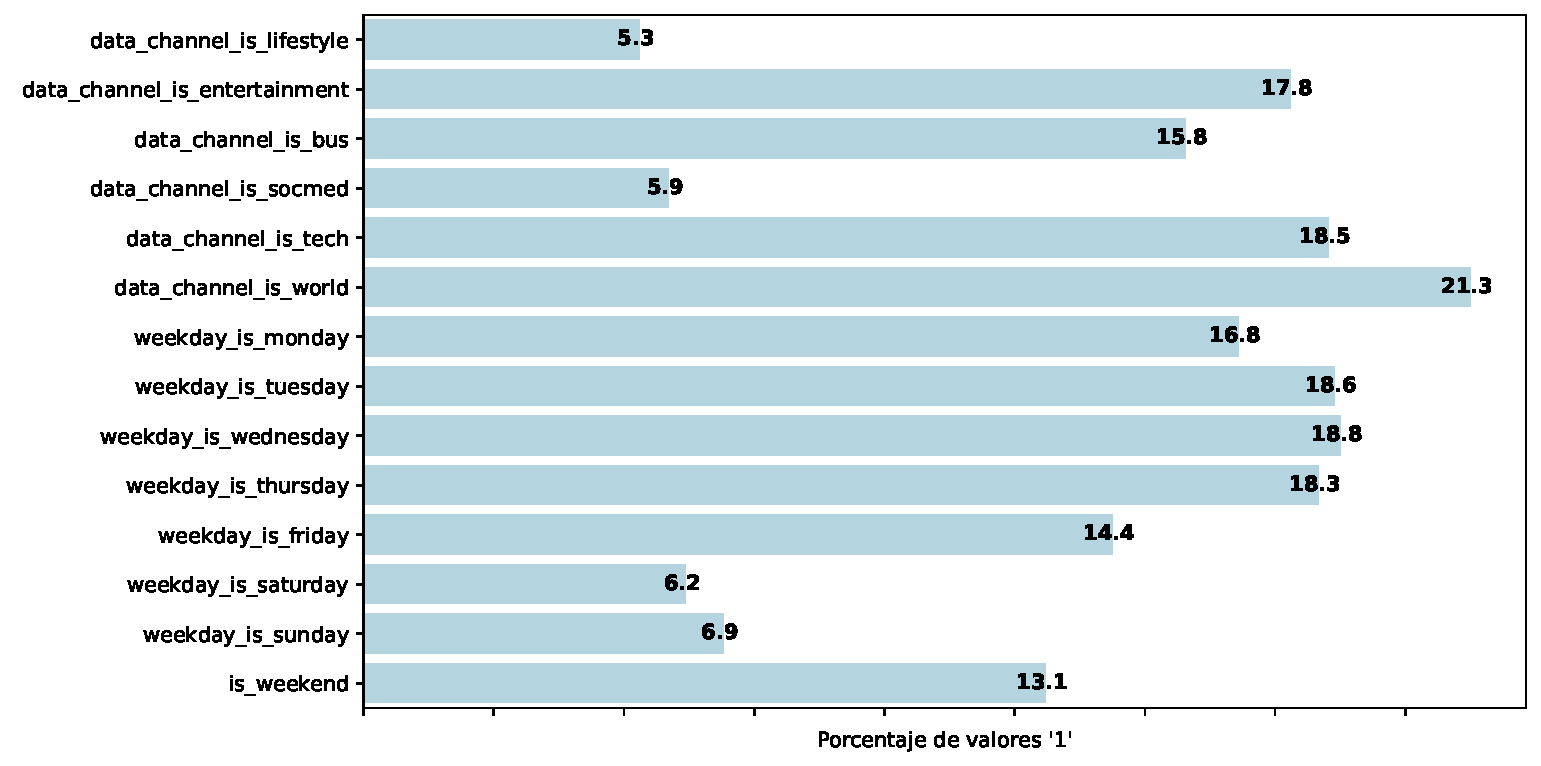
\includegraphics{Articulo_v2_files/figure-pdf/cell-4-output-1.pdf}

El conjunto de datos también presenta componentes de análisis semántico
latente y puntuaciones de sentimiento, capturando el tono emocional y la
objetividad del contenido. Las métricas de participación, como el número
de veces que se comparte y las referencias a sí mismo, son cruciales
para comprender el alcance e impacto del contenido. Todas estas son
variables continuas.

\subsection{Metodología}\label{metodologuxeda}

El presente trabajo prioriza la etapa de procesamiento del dataset, paso
fundamental antes de realizar el entrenamiento de los datos. El conjunto
de datos que actualmente manejamos cuenta con 58 características y 39
mil registros, por lo que claramente se observa la necesidad de reducir
el número de caracteristicas. Para un adecuado procesamiento y
entrenamiento de datos, el presente trabjo considera los sigientes
pasos: 1) Exploración y análisis de datos: en este paso realizaremos la
reducción de la dimensionalidad utilizando la herramienta de análisis de
principales componentes (PCA) y análisis de correlación de datos, ambos
métodos nos ayudaran a visualizar y entender las relaciones y patrones
de las variables. 2) Selección y entrenamiento del modelo: En este paso
utilizaremos varios modelos de clasificación, incluyendo
RandomForestClassifier \citep{breiman2001}, AdaBoostClassifier
\citep{freund1997}, LogisticRegression \citep{cox1958} y K-Nearest
Neighbors \citep{hodges1951}. Para optimizar los hiperparámetros y
mejorar el rendimiento de estos modelos se empleó GridSearchCV
\citep{pedregosa2011}, el cual realiza una búsqueda exhaustiva a través
de un rango especificado de valores de parámetros. Además, se consideró
el modelo GradientBoostingClassifier \citep{friedman2001}, un método de
boosting que, al igual que AdaBoost, combina múltiples modelos débiles
para formar un modelo fuerte. Estos enfoques maximizan la precisión y
robustez de las predicciones al ajustar finamente los parámetros y
combinar varios clasificadores en un esquema de ensamble. 3) Validación
y evaluación del modelo: en otras palabras, medir el rendimiento del
modelo utilizando datos de prueba y métricas de evaluación. Para ello,
se evaluará el rendimiento de los modelos mediante área bajo la curva
(AUC), una métrica que proporciona una medida agregada del rendimiento
en todas las posibles clasificaciones. 4) Finalmente se describirá los
resultados, interpretación y discusiones: en esta parte nos apoyaremos
mediante figuras y gráficos estadísticos y correlacionaremos con
anteriores resultados.

\subsubsection{Exploración y análisis de
datos}\label{exploraciuxf3n-y-anuxe1lisis-de-datos}

En la fase de exploración y análisis de datos, se comienza con el
ordenamiento de caracteres, que implica la normalización y limpieza de
los datos textuales, como la conversión a minúsculas, la eliminación de
espacios vacios y caracteres especiales. Luego, se procede a la
eliminación de características irrelevantes, identificando y descartando
aquellas que no aportan valor predictivo. A continuación, se realiza la
unión de variables, combinando múltiples características en una sola
para simplificar\\
el análisis. La creación de una matriz de correlación permite
identificar relaciones entre variables, ayudando a detectar
características redundantes. Finalmente, se aplica la disminución de
dimensionalidad, utilizando técnicas como el Análisis de Componentes
Principales (PCA), para reducir el número de características manteniendo
la mayor cantidad de información posible. Este proceso asegura que los
datos sean limpios, relevantes y manejables, facilitando el desarrollo
de modelos predictivos efectivos.

\subsubsection{Selección y entrenamiento del
modelo}\label{selecciuxf3n-y-entrenamiento-del-modelo}

\subsubsection{Clasificación Random
Forest}\label{clasificaciuxf3n-random-forest}

Los bosques aleatorios son métodos de aprendizaje en conjunto para la
regresión que utilizan múltiples árboles de decisión. El algoritmo
extrae muestras bootstrap del conjunto de datos original y genera
árboles de regresión no podados para cada muestra. En lugar de elegir el
mejor atributo de división, se selecciona aleatoriamente de un conjunto
de atributos. La predicción final se obtiene promediando las
predicciones de todos los árboles individuales. Se utilizó la librería
\href{https://scikit-learn.org/stable/modules/generated/sklearn.ensemble.RandomForestClassifier.html}{\texttt{scikit-learn}},
para implementar el modelo de Random Forest (bosque aleatorio) y fijamos
el número de estimadores en 50 estimadores con random\_state igual a 42.

\subsubsection{AdaBoostClassifier (Adaptive
Boosting)}\label{adaboostclassifier-adaptive-boosting}

Es un algoritmo de aprendizaje automático utilizado principalmente para
tareas de clasificación. AdaBoost funciona construyendo un modelo a
partir de un conjunto inicial de datos y luego ajusta iterativamente los
pesos de los ejemplos mal clasificados, incrementando la influencia de
aquellos que resultaron más difíciles de clasificar en cada iteración.
Esto permite que los clasificadores posteriores se centren más en los
ejemplos difíciles. Finalmente, los modelos individuales se combinan
mediante una votación ponderada para mejorar la precisión global.
AdaBoost es conocido por su capacidad para mejorar el rendimiento de
modelos débiles y su eficacia en diversos dominios, aunque su
rendimiento puede verse afectado por la presencia de ruido en los datos
y por la elección de los clasificadores base. Este modelo se implementó
utilizando la librería Scikit-learn.

\subsubsection{Regresión logística}\label{regresiuxf3n-loguxedstica}

La regresión logística es una técnica de clasificación utilizada para
predecir la probabilidad de pertenencia a una clase binaria. Utiliza la
función sigmoide para convertir una combinación lineal de variables
independientes en una probabilidad, y ajusta el modelo minimizando la
función de costo logloss. La implementación del modelo fue realizando la
librería scikit-learn.

\subsubsection{K-Nearest Neighbors (KNN)}\label{k-nearest-neighbors-knn}

El modelo K-Nearest Neighbors (KNN) es un algoritmo de aprendizaje
supervisado utilizado para clasificación y regresión. Clasifica una
observación basándose en las clases de sus K vecinos más cercanos, donde
K=10 en este caso, utilizando una medida de distancia como la
Euclidiana. En clasificación, asigna la clase más común entre los
vecinos, y en regresión, toma el promedio de los valores de los vecinos.
Es un método simple y no paramétrico que no hace suposiciones sobre la
distribución de los datos, y puede implementarse fácilmente en Python
usando la Libreria scikit-learn.

\subsubsection{GridSearchCV}\label{gridsearchcv}

En este análisis, se examinan diversos modelos de clasificación para
predecir la popularidad de noticias en línea utilizando el dataset de
Online News Popularity de Mashable. Se implementan cuatro modelos:
RandomForest, AdaBoost, LogisticRegression y K-Nearest Neighbors (KNN).
Para cada modelo, se definen conjuntos específicos de hiperparámetros y
se emplea GridSearchCV para realizar una búsqueda exhaustiva de los
mejores parámetros mediante validación cruzada. Una vez entrenados y
optimizados los modelos, se selecciona el mejor estimador y se evalúa su
rendimiento en un conjunto de prueba. La precisión obtenida en este
conjunto se utiliza para comparar la eficacia de cada modelo. Este
proceso automatiza la selección de hiperparámetros y facilita una
comparación objetiva entre diferentes algoritmos de clasificación,
proporcionando información valiosa sobre su desempeño en el contexto de
la popularidad de noticias en línea. En la tabla \ref{} se lista los
mejores hiperparametros por modelo.

\begin{longtable}[]{@{}lll@{}}

\caption{\label{tbl-hyperparams}Hiperparámetros probados para cada
modelo}

\tabularnewline

\toprule\noalign{}
\endhead
\bottomrule\noalign{}
\endlastfoot
model & hyper parameter & Valores \\
Random Forest & n\_estimators & {[}10, 20, 50, 100, 200, 400{]} \\
AdaBoost & n\_estimators & {[}10, 20, 50, 100, 200, 400{]} \\
Logistic Regression & penalty & {[}\textquotesingle l1\textquotesingle,
\textquotesingle l2\textquotesingle{]} \\
& C & {[}0.001, 0.01, 0.1, 1, 10{]} \\
& solver & {[}\textquotesingle liblinear\textquotesingle,
\textquotesingle saga\textquotesingle{]} \\
K-Nearest Neighbors (KNN) & n\_neighbors & {[}3, 5, 7, 9, 11, 13{]} \\
& weights & {[}\textquotesingle uniform\textquotesingle,
\textquotesingle distance\textquotesingle{]} \\
& algorithm & {[}\textquotesingle auto\textquotesingle,
\textquotesingle ball\_tree\textquotesingle,
\textquotesingle kd\_tree\textquotesingle,
\textquotesingle brute\textquotesingle{]} \\

\end{longtable}

\section{Experimentación y
resultados}\label{experimentaciuxf3n-y-resultados}

Los resultados muestran que RandomForest y AdaBoost son los modelos con
mejor rendimiento general, con AUC (Área bajo la curva ROC) de 0.7095 y
0.7030 respectivamente. RandomForest alcanza una precisión (Accuracy) de
0.6510 y una precisión positiva (Precision) de 0.6447, mientras que
AdaBoost logra 0.6488 y 0.6423 respectivamente en estas métricas.
LogisticRegression, aunque presenta un AUC de 0.6793, muestra una
precisión y precision positiva ligeramente más bajas en comparación con
los modelos de ensemble. Por otro lado, MLP (Perceptrón Multicapa)
muestra el rendimiento más bajo con un AUC de 0.5679 y una precisión de
0.5034, aunque destaca en recall (Sensibilidad) con 0.7427. Estos
resultados resaltan la capacidad superior de los modelos ensemble como
RandomForest y AdaBoost para la clasificación, especialmente en términos
de AUC y precisión global.

Los resultados de las métricas de evaluación para los diferentes modelos
se presentan en la Table~\ref{tbl-metricas}.

\begin{longtable}[]{@{}lllll@{}}

\caption{\label{tbl-metricas}Métricas de evaluación de modelos}

\tabularnewline

\toprule\noalign{}
\endhead
\bottomrule\noalign{}
\endlastfoot
Model & AUC & Accuracy & Precision & Recall \\
Random Forest & 0.7095 & 0.651 & 0.6447 & 0.6406 \\
AdaBoost & 0.703 & 0.6488 & 0.6423 & 0.6389 \\
Logistic Regression & 0.6793 & 0.635 & 0.6286 & 0.6231 \\
MLP & 0.5679 & 0.5034 & 0.4954 & 0.7427 \\

\end{longtable}

El gráfico de barras muestra la comparación de las métricas de AUC (Área
bajo la curva ROC) y Accuracy para cuatro modelos de clasificación:
RandomForest, AdaBoost, LogisticRegression y MLP (Perceptrón Multicapa).
Cada modelo está representado por barras de diferentes colores: azul
para AUC y verde para Accuracy. RandomForest y AdaBoost destacan con
altos valores de AUC y Accuracy, seguidos por LogisticRegression con
valores ligeramente inferiores. En contraste, MLP muestra un desempeño
más bajo en ambas métricas. Esta representación visual facilita la
comparación directa del rendimiento relativo de cada modelo en términos
de su capacidad predictiva y precisión.

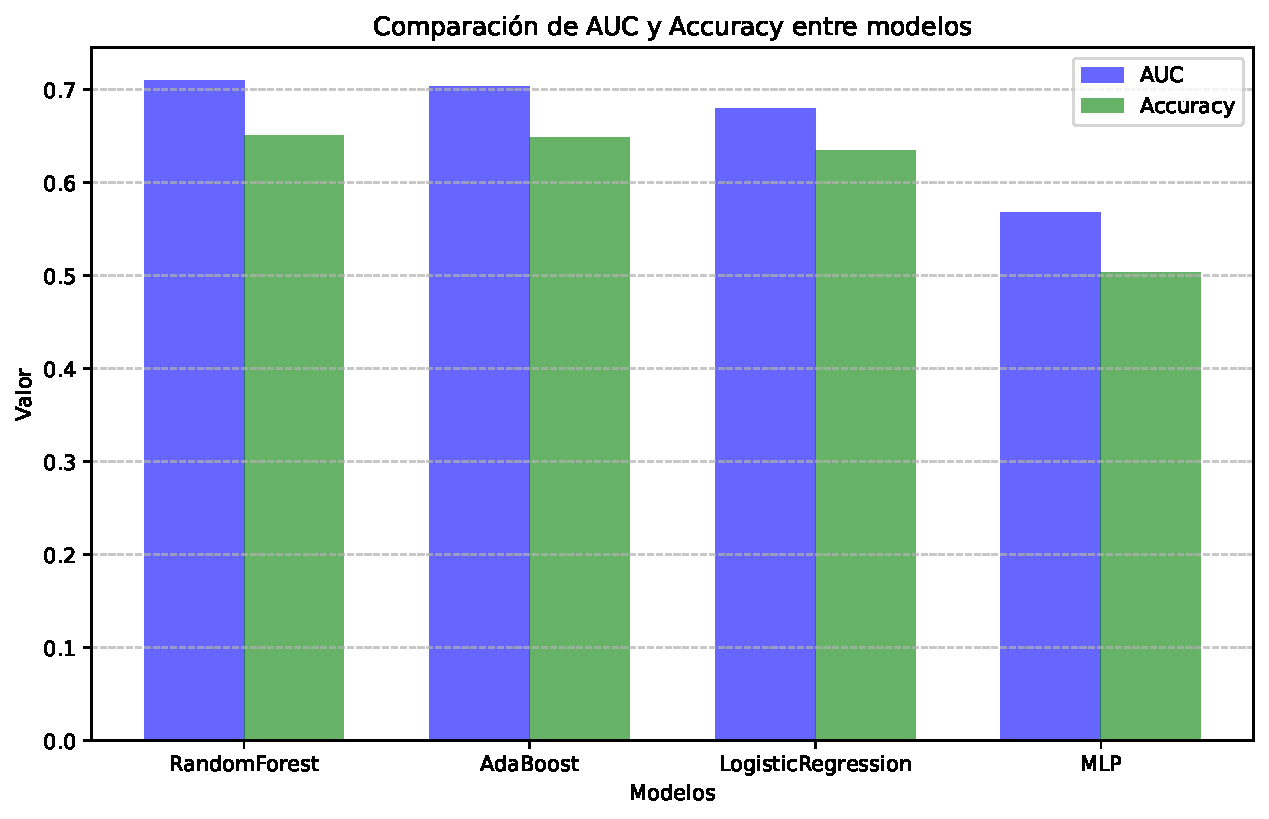
\includegraphics{Articulo_v2_files/figure-pdf/cell-9-output-1.pdf}

\section{Discusión}\label{discusiuxf3n}

\section{Conclusiones y trabajos
futuros}\label{conclusiones-y-trabajos-futuros}

Basado en las métricas evaluadas, los modelos RandomForest y AdaBoost
mostraron un rendimiento superior con AUC de 0.7095 y 0.7030
respectivamente, indicando una buena capacidad para clasificar
correctamente. LogisticRegression también fue competitivo con un AUC de
0.6793, aunque mostró una precisión ligeramente menor. En contraste, MLP
obtuvo un AUC más bajo de 0.5679, pero destacó en sensibilidad (recall)
con 0.7427, siendo efectivo en la identificación de casos positivos. En
conclusión, RandomForest y AdaBoost son recomendados por su sólido
desempeño general en este conjunto de datos, mientras que MLP muestra
una fortaleza en la detección de casos positivos.

En la siguiente etapa del trabajo, se tiene pensado implementar redes
neuronales como ejemplo Perceptrón Multicapa (Multilayer Perceptron,
MLP) para la clasificación de datos, el cual mejorara la predicción del
número de compartidos de las noticias de la página web
(www.mashable.com), explorando arquitecturas de redes neuronales más
complejas y variando el número de capas y neuronas para capturar mejores
patrones en datos complejos. Además, investigar funciones de activación
alternativas y técnicas de optimización avanzadas como ajuste dinámico
de hiperparámetros y regularización más efectiva podría aumentar la
eficiencia y precisión del modelo. Explorar técnicas como regularización
L1, dropout, y otras formas de optimización también sería beneficioso
para manejar problemas de sobreajuste y mejorar el rendimiento general
del ``Perceptrón Multicapa'' en la predicción de la popularidad de
noticias en plataformas online.


\renewcommand\refname{References}
  \bibliography{references.bib}


\end{document}
